% -*- root: ../mainThesis.tex -*-

\chapter{Constraint handling}
%
Let $\textbf{x}_{2k-1}$ and $\textbf{x}_{2k}$ be the coordinates of heel and 
toe of well $k$ respectively, and let $\boldsymbol{\xi}_{2k-1}$ and $\boldsymbol{\xi}_{2k-1}$
denote the initial coordinates (i.e., given as input) of heel and toe of well $k$. E.g., $\textbf{x}_{7}$
is the heel of well number four and $\boldsymbol{\xi}_{20}$ are the initial coordinates
of the toe of well number 10.\\
%
% ██╗    ██╗███████╗██╗     ██╗         ██╗     ███████╗███╗   ██╗ ██████╗████████╗██╗  ██╗
% ██║    ██║██╔════╝██║     ██║         ██║     ██╔════╝████╗  ██║██╔════╝╚══██╔══╝██║  ██║
% ██║ █╗ ██║█████╗  ██║     ██║         ██║     █████╗  ██╔██╗ ██║██║  ███╗  ██║   ███████║
% ██║███╗██║██╔══╝  ██║     ██║         ██║     ██╔══╝  ██║╚██╗██║██║   ██║  ██║   ██╔══██║
% ╚███╔███╔╝███████╗███████╗███████╗    ███████╗███████╗██║ ╚████║╚██████╔╝  ██║   ██║  ██║
%  ╚══╝╚══╝ ╚══════╝╚══════╝╚══════╝    ╚══════╝╚══════╝╚═╝  ╚═══╝ ╚═════╝   ╚═╝   ╚═╝  ╚═╝
%
\section{Well length constraint}
%
Since the well length constraints for the different wells are
independent of each other, we may compute their projections separately. 
Thus without loss of generality we may assume that $N=1$, that
is, we only deal with one well.

It is natural to assume that a well should have non-zero length
and that the total length of one well should be allowed to vary.
The distance between the heel and toe of a single well must be in the interval
$[L_{\min},L_{\max}]$. In other words they must be at least $L_{\min}$ apart
but not further away from each other than $L_{\max}$. From the previous assumptions
we get the constraints
%
\begin{equation}
\begin{aligned}
\| \textbf{x}_1 - \textbf{x}_2 \| &\geq L_{\min}, \\
\| \textbf{x}_1 - \textbf{x}_2 \| &\leq L_{\max}, 
\label{eq:well_length}
\end{aligned}
\end{equation}
%
where the lengths $L_{\max}$ and $L_{\min}$ satisfy $L_{\max} > L_{\min} > 0$.
If these conditions are not met by the initial input coordinates, $\boldsymbol{\xi}_{1}$ 
and $\boldsymbol{\xi}_{2}$ need to be projected back into feasible space by 
moving them as little as possible. This is done by solving
%
\begin{align}
	\min_{\textbf{x}_1,\textbf{x}_2 \in \mathbb{R}^3} f(\textbf{x}_1,\textbf{x}_2) =& \min_{\textbf{x}_1,\textbf{x}_2 \in \mathbb{R}^3}\left( \frac{1}{2} \| \textbf{x}_1 - \boldsymbol{\xi}_1 \|^2 + \frac{1}{2} \| \textbf{x}_2 - \boldsymbol{\xi}_2 \|^2 \right) \label{wlc_opt_1}\\
	 \intertext{subject to}																			
	h_1(\textbf{x}_1, \textbf{x}_2) =& +\frac{1}{2} \| \textbf{x}_1 - \textbf{x}_2 \|^2 - \frac{1}{2} L_{\min}^2 \geq 0, \label{wlc_opt_2}\\
    h_2(\textbf{x}_1, \textbf{x}_2) =& -\frac{1}{2} \| \textbf{x}_1 - \textbf{x}_2 \|^2 + \frac{1}{2} L_{\max}^2 \geq 0, \label{wlc_opt_3}
\end{align}
%
where the constraints have been squared so they can be differentiated.\\
%
There are three kinds of solutions depending on the configuration of the
initial positions of the heel and toe of the well. The initial positions $\boldsymbol{\xi}_1$
and $\boldsymbol{\xi}_2$ must either violate the $L_{\max}$ constraint, violate the
$L_{\min}$ constraint or they satisfy both constraints. The solution for each
initial configuration is given below and the proofs follow afterwards.\\
%
\begin{figure}[H]
	\centering
	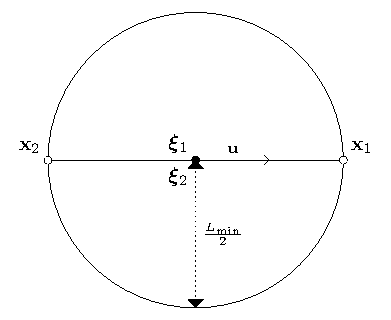
\includegraphics[]{figures/constraint_handling/well_length_zero.pdf}
	\caption{Minimum constraint violated. Initial points $\boldsymbol{\xi}_1, \boldsymbol{\xi}_2$ 
	are identical and solution points $\textbf{x}$ and $\textbf{y}$ lie on opposite sides of a circle 
	with radius $\frac{L_{\min}}{2}$. Note that the solution shown in the figure is only one of 
	the infinitely many solutions that exist for this case.}
	\label{fig:min_violation_zero}
\end{figure}
%
If $\| \boldsymbol{\xi}_1 - \boldsymbol{\xi}_2 \| < L_{\min}$ 
there are two solution types. If $\boldsymbol{\xi}_1 = \boldsymbol{\xi}_2$ 
then solutions are
%
\begin{equation}
\begin{aligned}
\textbf{x}_1 = \boldsymbol{\xi}_1 + \frac{L_{\min}}{2} \textbf{u}, \\
\textbf{x}_1 = \boldsymbol{\xi}_1 - \frac{L_{\min}}{2} \textbf{u},
\end{aligned}
\label{eq:solution_min_triv}
\end{equation}
%
for any vector $\textbf{u}$ of unit length. I.e., there is no unique solution and
all solutions are pairs of
points that lie on opposite sides of the circle with center $\boldsymbol{\xi}_1$ 
and radius $\frac{L_{\min}}{2}$. One such solution is shown in Figure
\ref{fig:min_violation_zero}.
%
\begin{figure}[H]
	\centering
	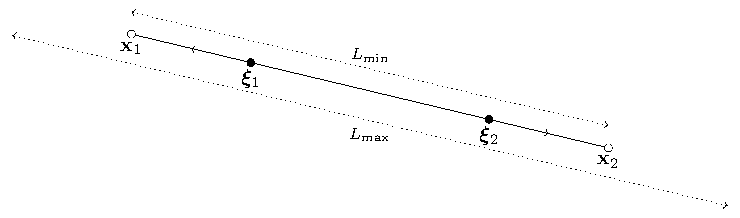
\includegraphics[]{figures/constraint_handling/well_length_min.pdf}
	\caption{Minimum constraint violated. Initial points $\boldsymbol{\xi}_1, \boldsymbol{\xi}_2$ 
	are too close and the solution is to move the points away from each other along the line that
	passes through them in opposite directions until the distance between them is exactly $L_{\min}$.}
	\label{fig:min_violation}
\end{figure}
%
If $\boldsymbol{\xi}_1 \neq \boldsymbol{\xi}_2$
then the solution is
%
\begin{equation}
\begin{aligned}
\textbf{x}_1 &= \boldsymbol{\xi}_1 + \frac{\lambda^*}{1 - 2\lambda^*} (\boldsymbol{\xi}_1 - \boldsymbol{\xi}_2), \\
\textbf{x}_2 &= \boldsymbol{\xi}_2 - \frac{\lambda^*}{1 - 2\lambda^*} (\boldsymbol{\xi}_1 - \boldsymbol{\xi}_2),
\end{aligned}
\label{eq:solution_min}
\end{equation}
were $ \lambda^* = \frac{1}{2} \left( 1 - \frac{\| \boldsymbol{\xi}_1 - \boldsymbol{\xi}_2 \|}{L_{\min}} \right)$.
Here both points are moved away from each other an equal distance along the line that passes through
$\boldsymbol{\xi}_1$ and $\boldsymbol{\xi}_2$ as shown in Figure \ref{fig:min_violation}.\\
%
%
\begin{figure}[H]
	\centering
	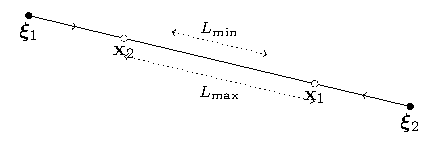
\includegraphics[]{figures/constraint_handling/well_length_max.pdf}
	\caption{Maximum constraint violated. Initial points $\boldsymbol{\xi}_1, \boldsymbol{\xi}_2$ 
	are too far away from each other and the solution is to move the points closer along the line 
	that passes through them until the distance between them is exactly $L_{\min}$.}
	\label{fig:max_violation}
\end{figure}
%
If $\| \boldsymbol{\xi}_1 - \boldsymbol{\xi}_2 \| > L_{\max}$
the solution is given by
\begin{equation}
\begin{aligned}
\textbf{x}_1 &= \boldsymbol{\xi}_1 - \frac{\mu^*}{1 + 2\mu^*} (\boldsymbol{\xi}_1 - \boldsymbol{\xi}_2), \\
\textbf{x}_2 &= \boldsymbol{\xi}_2 + \frac{\mu^*}{1 + 2\mu^*} (\boldsymbol{\xi}_1 - \boldsymbol{\xi}_2),
\end{aligned}
\label{eq:solution_max}
\end{equation}
where $\mu^* =\frac{1}{2} \left( \frac{\| \boldsymbol{\xi}_1 - \boldsymbol{\xi}_2 \|}{L_{\max}} - 1 \right) $. 
The geometric interpretation is that both points are moved closer to each other along the line that passes
through $\boldsymbol{\xi}_1$ and $\boldsymbol{\xi}_2$ as 
indicated in Figure \ref{fig:max_violation}.\\
%
\begin{figure}[H]
	\centering
	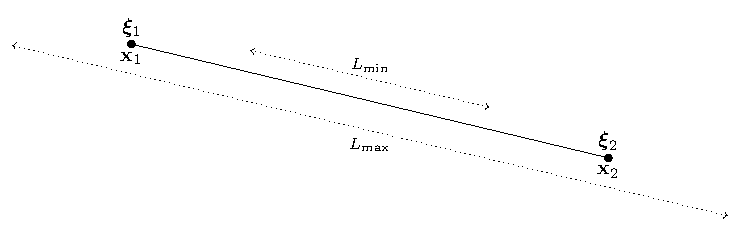
\includegraphics[]{figures/constraint_handling/well_length_feasible.pdf}
	\caption{Constraints are satisfied by initial points and no movement of the points is needed.}
	\label{fig:feasible}
\end{figure}
%
If $L_{\min} \leq \| \boldsymbol{\xi}_1 - \boldsymbol{\xi}_2 \| \leq L_{\max}$ the initial points
satisfy both constraints and as shown in 
Figure \ref{fig:feasible} we need not move them. 
The solution in this case is
\begin{equation}
\begin{aligned}
\textbf{x}_1 &= \boldsymbol{\xi}_1, \\
\textbf{x}_2 &= \boldsymbol{\xi}_2.
\label{eq:wl_formula_last}
\end{aligned}
\end{equation}
%
%
To prove the formulae \eqref{eq:solution_min_triv} -- \eqref{eq:wl_formula_last} 
consider the minimization problem \eqref{wlc_opt_1} -- \eqref{wlc_opt_3}, which can be 
solved by the method of Lagrange multipliers. Define the Lagrangian function
%
\begin{equation}
\begin{aligned}
\mathcal{L} (\textbf{x}_1,\textbf{x}_2,\lambda,\mu) &= \frac{1}{2} \| \textbf{x}_1 - \boldsymbol{\xi}_1 \|^2 + \frac{1}{2} \| \textbf{x}_2 - \boldsymbol{\xi}_2 \|^2 \\
&- \lambda \left( \frac{1}{2} \| \textbf{x}_1 - \textbf{x}_2 \|^2 - \frac{1}{2} L_{\min}^2 \right ) - \mu  \left( - \frac{1}{2} \| \textbf{x}_1 - \textbf{x}_2 \|^2 + \frac{1}{2} L_{\max}^2 \right ),
\end{aligned}
\label{lagrangeFunc}
\end{equation}
%
where $\lambda, \mu \in \mathbb{R}$ are the Lagrange multipliers for the constraints.
Note that only one of the constraints can be active at once, meaning that either $\lambda$
or $\mu$ must be zero.\\
A necessary condition for a local minimum $\textbf{x}_1^*, \textbf{x}_2^*$ is that 
it satisfies the first order KKT conditions
%
\begin{equation}
\begin{aligned}
\nabla_{\textbf{x}_1,\textbf{x}_2} \mathcal{L} (\textbf{x}_1^*, \textbf{x}_2^*, \lambda^*, \mu^*) &= 0, \\
\lambda h_1(\textbf{x}_1^*, \textbf{x}_2^*) &= 0,\\
\mu h_2(\textbf{x}_1^*, \textbf{x}_2^*) &= 0,\\
\lambda &\geq 0,\\
\mu &\geq 0,\\
h_i(\textbf{x}_1^*, \textbf{x}_2^*) &\geq 0, \qquad  i=1,2. \\
\end{aligned}
\end{equation}
%
Differentiating the Lagrangian and setting the gradient to 0 we obtain the system of equations
\begin{equation}
\begin{aligned}
\nabla_{\textbf{x}_1} \mathcal{L} &= \textbf{x}_1 - \boldsymbol{\xi}_1 - \lambda ( \textbf{x}_1 - \textbf{x}_2 ) + \mu ( \textbf{x}_1 - \textbf{x}_2 ) = 0, \\
\nabla_{\textbf{x}_2} \mathcal{L} &= \textbf{x}_2 - \boldsymbol{\xi}_2 + \lambda ( \textbf{x}_1 - \textbf{x}_2 ) - \mu ( \textbf{x}_1 - \textbf{x}_2 ) = 0. \\
\end{aligned}
\label{eq:gradients}
\end{equation}
%
%
The problem is solved by dividing the positions of the initial points, $\boldsymbol{\xi}_1 $ 
and $\boldsymbol{\xi}_2$ into three different cases and then considering different candidate 
solutions $(\textbf{x}_1^*, \textbf{x}_2^*, \lambda^*, \mu^*)$. The three different categories
for the initial position of the heel and toe of the well must either violate exactly one of the
constraints, or violate none of them. The optimal solution of a configuration must satisfy the
constraints, i.e., $L_{\min} \leq \| \textbf{x}_1^* - \textbf{x}_2^* \| \leq L_{\max}$. A solution
must satisfy exactly one of the following equations
%
\begin{equation}
\begin{aligned}
L_{\min} < \| \textbf{x}_1^* - \textbf{x}_2^* \| &< L_{\max}, \\
\| \textbf{x}_1^* - \textbf{x}_2^* \| &= L_{\min}, \\
\| \textbf{x}_1^* - \textbf{x}_2^* \| &= L_{\max}.
\label{eq:intercategories}
\end{aligned}
\end{equation}
%
For each of the three cases for the initial positions of the well we will
consider each of the three possibilities for the solution.
%
\subsection{Case 1. Initial points feasible}
%
Assume that $ L_{\min} \leq \| \boldsymbol{\xi}_1 - \boldsymbol{\xi}_2 \| \leq L_{\max} $.
Then the initial points satisfy the distance constraint and no movement of the points is needed. 
Because the objective function $f$ is non-negative
and $f(\boldsymbol{\xi}_1,\boldsymbol{\xi}_2) = 0$ this solution is the global minimum.
%
%
\subsection{Case 2. Initial points too close}
%
Assume that $ \| \boldsymbol{\xi}_1 - \boldsymbol{\xi}_2 \| < L_{\min} $.
The distance between the initial points is too small and must be increased.
%
According to \eqref{eq:intercategories} there are three different possibilities 
for the distance between the candidate solutions $\textbf{x}_1^*, \textbf{x}_2^*$. 
%
If 
\begin{equation}
L_{\max} >  \| \textbf{x}_1^* - \textbf{x}_2^*  \| > L_{\min},
\label{eq:interior}
\end{equation}
i.e., the solution lies in the interior of both constraints. 
Then none of the constraints are active, which gives
$\lambda^* =\mu^* = 0 $ and therefore
%
\begin{equation}
\begin{aligned}
    	\textbf{x}_1^* &= \boldsymbol{\xi}_1,\\
    	\textbf{x}_2^* &= \boldsymbol{\xi}_2.
\end{aligned}
\end{equation}
%
But this results in the contradiction 
$\| \textbf{x}_1^* - \textbf{x}_2^*  \| = \| \boldsymbol{\xi}_1 - \boldsymbol{\xi}_2 \| \leq L_{\min},$ 
and thus the solution cannot satisfy \eqref{eq:interior}.\\
%
%
If $\| \textbf{x}_1^* - \textbf{x}_2^*  \| = L_{\min}$, the maximum
constraint is inactive which means that $\mu = 0$. Inserting this into 
equation \eqref{eq:gradients} gives
%
\begin{equation}
\begin{aligned}
\textbf{x}_1 - \boldsymbol{\xi}_1 - \lambda ( \textbf{x}_1 - \textbf{x}_2 )  &= 0, \\
\textbf{x}_2 - \boldsymbol{\xi}_2 + \lambda ( \textbf{x}_1 - \textbf{x}_2 )  &= 0,
\end{aligned}
\label{eq:gradients_2.1}
\end{equation}
%
which is a linear system with respect to $\textbf{x}_1$ and $\textbf{x}_2$.
Now if $\boldsymbol{\xi}_1 = \boldsymbol{\xi}_2$, which means the initial well has zero length,
then it follows that $\lambda=\frac{1}{2}$ and we get
%
\begin{align}
\textbf{x}_1 + \textbf{x}_2 &= 2 \boldsymbol{\xi}_1, \\
\| \textbf{x}_1^* - \textbf{x}_2^*\| &= L_{\min}.
\label{eq:zero_length_solution}
\end{align}
%
This equation has solutions
\begin{align}
\textbf{x}_1 = \boldsymbol{\xi}_1 + \frac{L_{\min}}{2} \textbf{u} , \\
\textbf{x}_1 = \boldsymbol{\xi}_1 - \frac{L_{\min}}{2} \textbf{u} ,
\label{eq:zero_length_solutions}
\end{align}
for all unit vectors $\textbf{u}$ and they are all KKT points. So if the initial 
well has zero length the solutions all lie on a circle with center $\boldsymbol{\xi}_2$ 
and radius $\frac{L_{\min}}{2}$.
%
Now if $\boldsymbol{\xi}_1 \neq \boldsymbol{\xi}_2$, then 
solving the system \eqref{eq:gradients_2.1} gives
%
\begin{equation}
\begin{aligned}
\textbf{x}_1 &=  \frac{1}{(1-\lambda)^2 -(\lambda)^2 } \left( (1-\lambda) \boldsymbol{\xi}_1 - \lambda \boldsymbol{\xi}_2 \right) 
= \boldsymbol{\xi}_1 + \frac{\lambda}{1 - 2\lambda} (\boldsymbol{\xi}_1 - \boldsymbol{\xi}_2), \\
\textbf{x}_2 &=  \frac{1}{(1-\lambda)^2 -(\lambda)^2 } \left(-\lambda \boldsymbol{\xi}_1 + (1-\lambda) \boldsymbol{\xi}_2 \right)
= \boldsymbol{\xi}_2 - \frac{\lambda}{1 - 2\lambda} (\boldsymbol{\xi}_1 - \boldsymbol{\xi}_2).
\end{aligned}
\label{eq:solutions_2.2}
\end{equation}
%
Combining this result with the condition that $\| \textbf{x}_1^* - \textbf{x}_2^*\| = L_{\min}$ we obtain
%
\begin{equation}
\lambda^* = \frac{1}{2} \left( 1 \pm \frac{\| \boldsymbol{\xi}_1 - \boldsymbol{\xi}_2 \|}{L_{\min}} \right),
\label{eq:solutions_lambda_2.2}
\end{equation}
%
where both candidates for $\lambda^*$ are positive and therefore yield KKT points.
From \eqref{eq:gradients_2.1} we have
%
\begin{equation}
f(\textbf{x}_1,\textbf{x}_2) = \lambda^2 \| \textbf{x}_1 - \textbf{x}_2\|^2,
\label{eq:well_length_min}
\end{equation}
%
and thus the minimum is attained for the smaller candidate. The best KKT point is therefore given by

\begin{equation}
\begin{aligned}
\textbf{x}_1^* &= \boldsymbol{\xi}_1 + \frac{\lambda^*}{1 - 2\lambda^*} (\boldsymbol{\xi}_1 - \boldsymbol{\xi}_2), \\
\textbf{x}_2^* &= \boldsymbol{\xi}_2 - \frac{\lambda^*}{1 - 2\lambda^*} (\boldsymbol{\xi}_1 - \boldsymbol{\xi}_2),
\label{eq:best_min}
\end{aligned}
\end{equation}
where 
$\lambda^* = \frac{1}{2} \left( 1 - \frac{\| \boldsymbol{\xi}_1 - \boldsymbol{\xi}_2 \|}{L_{\min}} \right).$
%
%

The last possibility is that $L_{\max} =  \| \textbf{x}_1^* - \textbf{x}_2^*  \|$.
%
The derivation is similar to the previous case.
The maximum constraint is active so therefore the other
constraint is inactive and hence $\lambda = 0.$
If $\boldsymbol{\xi}_1 = \boldsymbol{\xi}_2$ then we get infinitely 
many solutions
%
\begin{align}
\textbf{x}_1 + \textbf{x}_2 &= 2 \boldsymbol{\xi}_1, \\
\| \textbf{x}_1^* - \textbf{x}_2^*\| &= L_{\max},
\label{eq:zero_length_solution_max}
\end{align}
%
but since these all lie on a circle with center in $\boldsymbol{\xi}_1$ and radius
$\frac{L_{\max}}{2}$ the solutions are all worse than the ones in \eqref{eq:zero_length_solutions}
so none of them can be a global minimum.
%
\begin{equation}
\begin{aligned}
\textbf{x}_1 =  \frac{1}{(1+\mu)^2 -(\mu)^2 } \left( (1+\mu) \boldsymbol{\xi}_1 + \mu \boldsymbol{\xi}_2 \right) 
= \boldsymbol{\xi}_1 - \frac{\mu}{1+2 \mu} (\boldsymbol{\xi}_1 - \boldsymbol{\xi}_2), \\
\textbf{x}_2 =  \frac{1}{(1+\mu)^2 -(\mu)^2 } \left( \mu \boldsymbol{\xi}_1 + (1+\mu) \boldsymbol{\xi}_2 \right)
= \boldsymbol{\xi}_2 + \frac{\mu}{1+2 \mu} (\boldsymbol{\xi}_1 - \boldsymbol{\xi}_2).
\end{aligned}
\label{eq:solutions_2.3}
\end{equation}
%
Using the fact that $L_{\max} =  \| \textbf{x}_1^* - \textbf{x}_2^*  \|$ 
and solving for $\mu$ results in
%
\begin{equation}
\mu = - \frac{1}{2} \left( 1 \pm \frac{\| \boldsymbol{\xi}_1 - \boldsymbol{\xi}_2 \|}{L_{\max}} \right) < 0,
\label{eq:solutions_mu_2.3}
\end{equation}
%
which are not solutions since the Lagrange multiplier in both cases is negative.
Now it follows that, since there are only two points that satisfy the KKT
conditions, the better one has to be the global optimum, and thus the
solution for Case 2 is given by \eqref{eq:best_min}
%
%
\subsection{Case 3. Initial points too distant}
%
The initial condition is that $ \| \boldsymbol{\xi}_1 - \boldsymbol{\xi}_2 \| > L_{\max}$,
which means that the initial points are too far away from each other and need to
be moved closer to each other.
The solutions for this case are analogous to Case 2 and the calculations 
will be omitted. The only valid solution is found when
$\| \textbf{x}_1^* - \textbf{x}_2^*  \| = L_{\max}$ which results in
$\mu^* = \frac{1}{2} \left( - 1 + \frac{\| \boldsymbol{\xi}_1 - \boldsymbol{\xi}_2 \|}{L_{\max}} \right)$
and $\lambda^* = 0$. This gives the solution 
\begin{equation}
\begin{aligned}
\textbf{x}_1^* &= \boldsymbol{\xi}_1 - \frac{\mu^*}{1 + 2\mu^*} (\boldsymbol{\xi}_1 - \boldsymbol{\xi}_2), \\
\textbf{x}_2^* &= \boldsymbol{\xi}_2 + \frac{\mu^*}{1 + 2\mu^*} (\boldsymbol{\xi}_1 - \boldsymbol{\xi}_2).
\end{aligned}
\end{equation}

%
%
%
% ██╗███╗   ██╗████████╗███████╗██████╗     ██╗    ██╗███████╗██╗     ██╗         ██████╗ ██╗███████╗████████╗ █████╗ ███╗   ██╗ ██████╗███████╗
% ██║████╗  ██║╚══██╔══╝██╔════╝██╔══██╗    ██║    ██║██╔════╝██║     ██║         ██╔══██╗██║██╔════╝╚══██╔══╝██╔══██╗████╗  ██║██╔════╝██╔════╝
% ██║██╔██╗ ██║   ██║   █████╗  ██████╔╝    ██║ █╗ ██║█████╗  ██║     ██║         ██║  ██║██║███████╗   ██║   ███████║██╔██╗ ██║██║     █████╗  
% ██║██║╚██╗██║   ██║   ██╔══╝  ██╔══██╗    ██║███╗██║██╔══╝  ██║     ██║         ██║  ██║██║╚════██║   ██║   ██╔══██║██║╚██╗██║██║     ██╔══╝  
% ██║██║ ╚████║   ██║   ███████╗██║  ██║    ╚███╔███╔╝███████╗███████╗███████╗    ██████╔╝██║███████║   ██║   ██║  ██║██║ ╚████║╚██████╗███████╗
% ╚═╝╚═╝  ╚═══╝   ╚═╝   ╚══════╝╚═╝  ╚═╝     ╚══╝╚══╝ ╚══════╝╚══════╝╚══════╝    ╚═════╝ ╚═╝╚══════╝   ╚═╝   ╚═╝  ╚═╝╚═╝  ╚═══╝ ╚═════╝╚══════╝
\section{Inter-well distance constraint}
%
Minimize the movement of the endpoints of two line 
segments such that every point on the first 
line segment is at least some distance $d$ away 
from every point on the other line segment.
%
Let the initial positions of the two line segments be 
defined by their endpoints 
$\boldsymbol{\xi}_1, \boldsymbol{\xi}_2, \boldsymbol{\xi}_3, \boldsymbol{\xi}_4 \in \mathbb{R}^3$ 
respectively. Minimizing the movement is the solution to the problem
%
\begin{equation}
\min_{ \textbf{x}_i \in \mathbb{R}^3 } F(\textbf{x}_1,\textbf{x}_2,\textbf{x}_3,\textbf{x}_4) = \min_{ \textbf{x}_i \in \mathbb{R}^3 } \sum_{i=1}^4 \frac{1}{2} \| \textbf{x}_i - \boldsymbol{\xi}_i \|^2
\label{eq:interwell_distance}
\end{equation}
under the conditions that
\begin{align}
c(\textbf{x}_1,\textbf{x}_2,\textbf{x}_3,\textbf{x}_4,\lambda_1,\lambda_2) \geq \frac{1}{2} d^2\label{eq:interwell_distance_constraint}\\
\intertext{for all} 
\quad \lambda_i \in [0,1], \quad i=1,2,	\label{eq:interwell_distance_lambda}
\end{align}
%
where
%
\begin{equation}
c(\textbf{x}_1,\textbf{x}_2,\textbf{x}_3,\textbf{x}_4,\lambda_1,\lambda_2) = 
\frac{1}{2} \| (\textbf{x}_1 + \lambda_1 (\textbf{x}_2 - \textbf{x}_1 )) - (\textbf{x}_3 + \lambda_2 (\textbf{x}_4 - \textbf{x}_3)) \|^2.
\end{equation}
%
Call a solution in which $k$ points are moved a $k$-point solution. We will first
try to solve \eqref{eq:interwell_distance} -- \eqref{eq:interwell_distance_lambda} by
moving only two points, then by moving just three points, and lastly, if a solution is
not yet found, move all four points. The idea is that, if the optimal solution for
moving two or three points while temporarily ignoring the other point(s) satisfies all
the constraints in \eqref{eq:interwell_distance_lambda}, then this must be the 
optimal solution to \eqref{eq:interwell_distance}. \\
%
To see why this is true, notice that in general if $\Omega_1 \subset \Omega_2$,
then
\begin{align}
\min_{x \in \Omega_1} f(x) \geq \min_{x \in \Omega_2} f(x)
\label{eq:set_min}
\end{align}
holds for all real valued functions $f$. Thus if we have that
%
\begin{align}
 f(x^*) = \min_{x \in \Omega_2} f(x) \quad \text{and} \quad x^* \in \Omega_1,
\end{align}
%
then $x^*$ is feasible for the first problem and 
%
\begin{align}
f(x^*) \leq f(x) \quad \forall x \in \Omega_1,
\end{align}
%
which means that $x^*$ is the solution to both minimization problems, i.e.,
%
\begin{align}
\min_{x \in \Omega_1} f(x) = \min_{x \in \Omega_2} f(x) = f(x^*).
\label{eq:set_min_end}
\end{align}
% 
Now ignoring one of the four points is the same as setting either $\lambda_1$ or
$\lambda_2$ equal to 1 or 0 in \eqref{eq:interwell_distance_lambda}. E.g., if we
wish to only consider the points $\textbf{x}_1, \textbf{x}_2$ and $\textbf{x}_4$
but ignore $\textbf{x}_3$ this is done by letting $\lambda_2 = 1$. Call the set
of feasible points for a $k$-point problem $\tilde{\Omega}_k$. Clearly we must
have $\tilde{\Omega}_4 \subset \tilde{\Omega}_3 \subset \tilde{\Omega}_2 \subset \tilde{\Omega}_1$. Then by 
\eqref{eq:set_min} -- \eqref{eq:set_min_end} we have that the $k$-point solution 
with the smallest value for $k$ which is feasible in the four point problem, 
must also be the solution to the four point problem.

%
\subsection[Number of points moved]{Number of points moved and form of solutions}
%
A line segment that connects the two solution line segments, $S_1, S_2$, over the 
shortest distance will be called SD (Shortest Distance). If only one of the two line 
segments is needed in a figure then, without loss of generality, we will refer to this
line segment as $S_1$ with endpoints $\textbf{x}_1$ and $\textbf{x}_2$. Divide the solutions of the
problem into different categories depending on how many of the points have been moved. 
Denote the smallest angle between the SD and $S_i$ by $\alpha_i$. Note that SD is not
unique if $S_1$ and $S_2$ are parallel, but the angles $\alpha_1$ and $\alpha_2$ are.
We must also have that $\alpha_i \geq 90^\circ$. If one angle is below $90^\circ$ then there 
exists a shorter distance between the line segments by moving the SD along 
the line segment in the direction of the angle as indicated by the arrow
in Figure \ref{fig:four_point_all_alpha}. 
%
\begin{figure}[H]
	\centering
	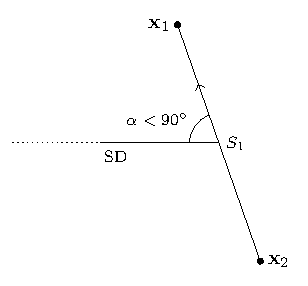
\includegraphics[width=0.45\textwidth]{figures/constraint_handling/interwell_angles.pdf}
	\caption{Candidate for shortest distance (SD). A shorter distance between the segments
			 can be found by moving upwards along the line segment.}
	\label{fig:four_point_all_alpha}
\end{figure}
%
%
If one angle $\alpha$ is over 90 degrees, then the SD must connect to an endpoint
of the corresponding line segment (or else SD could be improved by moving it along the line
segment) as shown in Figure \ref{fig:four_point_angles_4p}. 
%
\begin{figure}[H]
	\centering
	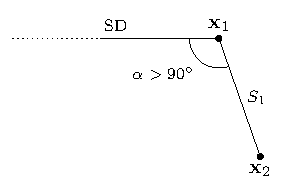
\includegraphics[width=0.45\textwidth]{figures/constraint_handling/interwell_angles_4p.pdf}
	\caption{One angle over 90 degrees. Moving $\textbf{x}_2$ does not change the length of SD.}
	\label{fig:four_point_angles_4p}
\end{figure}
%
Assume that this is the case.
Without loss of generality we call this endpoint $\textbf{x}_1$ and the other endpoint of
the line segment $\textbf{x}_2$. Then moving $\textbf{x}_2$ a small distance does not
change the shortest distance. It follows that $\textbf{x}_2 = \boldsymbol{\xi}_2$ because
no constraints are active for $\textbf{x}_2$ and this cannot be a solution where all four
points have been moved. Therefore, in a solution where all four points are moved,
both of the angles must be 90 degrees.
%
If we have a case where both angles are over 90 degrees as shown in
Figure \ref{fig:four_point_angles_3p}, then the SD connects two
endpoints,
%
\begin{figure}[H]
	\centering
	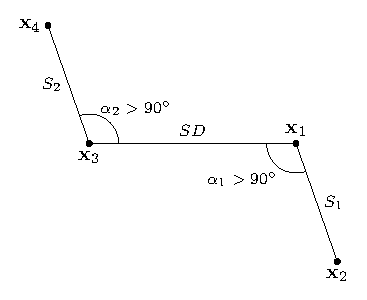
\includegraphics[width=0.45\textwidth]{figures/constraint_handling/interwell_angles_3p.pdf}
	\caption{One angle over 90 degrees}
	\label{fig:four_point_angles_3p}
\end{figure}
%
\noindent and by applying the same argument as above to 
both line segments we see this is a solution where at most
two points have been moved. Thus it cannot be a three-point solution.
Therefore a three-point solution must have one angle $\alpha$
equal to $90^{\circ}$ and the other one larger than $90^{\circ}$.
%
If we are left with both angles larger than $90^{\circ}$ then we must have moved either
two points or no points.
%
\subsection{Four-point solution}
%
Denote the initial points $\boldsymbol{\xi}_1, \boldsymbol{\xi}_2, \boldsymbol{\xi}_3$ 
and $\boldsymbol{\xi}_4$ and the solution points $\textbf{x}_1, \textbf{x}_2, \textbf{x}_3$ 
and $\textbf{x}_4$. In the solution the SD will be orthogonal to both line segments. 
This means that in the solution the line segments will lie in two planes $E^1$ and $E^2$
that share the same normal vector (namely SD). This means that $E^1$ and $E^2$ are parallel 
and a distance $d$ apart. 
Let
%
\begin{equation}
E^0 = E_{\textbf{s},t} = \{ \textbf{x} : \langle \textbf{s},\textbf{x} \rangle = t \}
\end{equation} 
be the plane that lies between the two solution planes with $\textbf{s}$ the
normalized SD vector (pointing towards the line segment with endpoints $\textbf{x}_1, \textbf{x}_2$)
and $t \in \mathbb{R}$.
%
\begin{figure}[H]
	\centering
	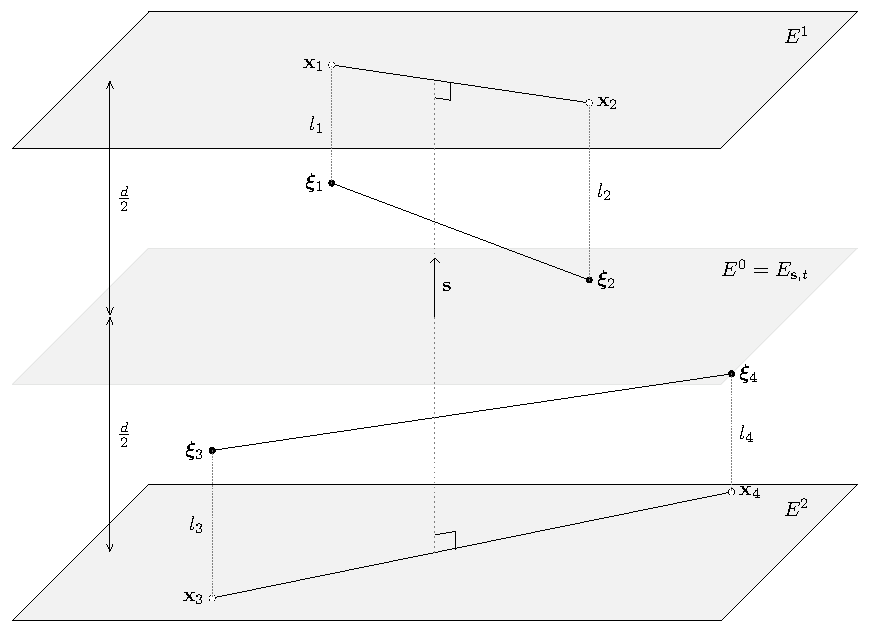
\includegraphics[width=0.95\textwidth]{figures/constraint_handling/four_point_interwell_problem.pdf}
	\caption{Four point solution. All four initial points have been moved and the resulting shortest distance
			 line is orthogonal to both solutions. Project initial points down on planes to get the optimal
			 solution.}
	\label{fig:four_point_problem}
\end{figure}
%
If the two planes $E^1$ and $E^2$ are found, then the solution is simply
the shortest distance from the initial points to the planes, which is found by projecting 
$\textbf{x}_1$ and $\textbf{x}_2$ onto $E^1 = E_{\textbf{s},t+\frac{d}{2}}$ and by projecting
$\textbf{x}_3$ and $\textbf{x}_4$ onto $E^2 = E_{\textbf{s},t-\frac{d}{2}}$.
%
Denote
%
\begin{equation}
\begin{aligned}
l_1(\textbf{s},t) &=  \langle \textbf{s}, \boldsymbol{\xi}_1 \rangle - t  - \frac{d}{2}, \\
l_2(\textbf{s},t) &=  \langle \textbf{s}, \boldsymbol{\xi}_2 \rangle - t  - \frac{d}{2}, \\
l_3(\textbf{s},t) &=  \langle \textbf{s}, \boldsymbol{\xi}_3 \rangle - t  + \frac{d}{2}, \\
l_4(\textbf{s},t) &=  \langle \textbf{s}, \boldsymbol{\xi}_4 \rangle - t  + \frac{d}{2},
\label{eq:interwell_lengths} 
\end{aligned}
\end{equation}
%
then $|l_i(\textbf{s},t)| = \| \textbf{x}_i - \boldsymbol{\xi}_i \|$.
Thus we can rewrite the minimization problem \eqref{eq:interwell_distance} 
and solve for $\textbf{s}$ and $t$ by
%
\begin{equation}
\min_{ \textbf{x}_i \in \mathbb{R}^3 } F(\textbf{x}_1,\textbf{x}_2,\textbf{x}_3,\textbf{x}_4) 
= \min_{ \textbf{s} \in \mathbb{S}^2, t \in \mathbb{R}} \frac{1}{2}  \sum_{i=1}^4 l_i(\textbf{s},t)^2.
\label{eq:interwell_st}
\end{equation}
%
Holding $\textbf{s}$ fixed and minimizing $F$ with respect to $t$ gives
the condition
%
\begin{align}
\frac{\partial F}{\partial t} (\textbf{s},t) =  
   &\langle \textbf{s},\boldsymbol{\xi}_1 \rangle - t  - \frac{d}{2} 
+  \langle \textbf{s},\boldsymbol{\xi}_2 \rangle - t  - \frac{d}{2} \\
&+ \langle \textbf{s},\boldsymbol{\xi}_3 \rangle - t  + \frac{d}{2} 
+  \langle \textbf{s},\boldsymbol{\xi}_4 \rangle - t  + \frac{d}{2} \\
= &\sum_{i=1}^4 \langle \boldsymbol{\xi}_i,\textbf{s} \rangle - 4t = 0, \\
\intertext{and therefore} 
t = &\frac{1}{4} \sum_{i=1}^4 \langle \boldsymbol{\xi}_i,\textbf{s} \rangle.
\end{align}
%
We simplify the problem by introducing the shifted variables
\begin{equation}
\hat{\boldsymbol{\xi}}_i = \boldsymbol{\xi}_i - \frac{1}{4} \sum_{i=1}^4 \boldsymbol{\xi}_i.
\end{equation}
%
We then get the identity
%
\begin{equation}
\begin{aligned}
\langle \textbf{s},\boldsymbol{\xi}_i \rangle   &= \langle \textbf{s},\hat{\boldsymbol{\xi}}_i \rangle
												+  \langle \textbf{s},\boldsymbol{\xi}_i - \hat{\boldsymbol{\xi}}_i \rangle\\
										        &= \langle \textbf{s},\hat{\boldsymbol{\xi}}_i \rangle 
										       	+  \Big\langle \textbf{s}, \frac{1}{4} \sum_{i=1}^4 \boldsymbol{\xi}_i \Big\rangle\\
												&= \langle \textbf{s},\hat{\boldsymbol{\xi}}_i \rangle
												+  \frac{1}{4} \sum_{i=1}^4 \langle \textbf{s},\boldsymbol{\xi}_i \rangle.
\end{aligned}												  
\end{equation}
%
For the shifted variables inserted into \eqref{eq:interwell_lengths} 
the variable $t$ is eliminated and equation \eqref{eq:interwell_st} 
can be rewritten as
%
\begin{equation}
\min_{ \textbf{s} \in \mathbb{S}^2, t \in \mathbb{R}} F(\textbf{s},t)=\min_{ \textbf{s} \in \mathbb{S}^2} \frac{1}{2}  \sum_{i=1}^4 \hat{l}_i(\textbf{s})^2
\end{equation}
%
with
%
\begin{equation}
\begin{aligned}
\hat{l}_1(\textbf{s},t) &=  \langle \textbf{s},\hat{\boldsymbol{\xi}}_1 \rangle - \frac{d}{2}, \\
\hat{l}_2(\textbf{s},t) &=  \langle \textbf{s},\hat{\boldsymbol{\xi}}_2 \rangle - \frac{d}{2}, \\
\hat{l}_3(\textbf{s},t) &=  \langle \textbf{s},\hat{\boldsymbol{\xi}}_3 \rangle + \frac{d}{2}, \\
\hat{l}_4(\textbf{s},t) &=  \langle \textbf{s},\hat{\boldsymbol{\xi}}_4 \rangle + \frac{d}{2}.
\label{eq:interwell_lengths_trans} 
\end{aligned}
\end{equation}
%
We differentiate $F$ with respect to $\textbf{s}$ to get
%
\begin{equation}
\frac{\partial F}{\partial \textbf{s}} (\textbf{s}) =  \sum_{i=1}^4 (\hat{\boldsymbol{\xi}}_i \otimes \hat{\boldsymbol{\xi}}_i)\textbf{s}
- \frac{d}{2}(\hat{\boldsymbol{\xi}}_1 + \hat{\boldsymbol{\xi}}_2) + \frac{d}{2}(\hat{\boldsymbol{\xi}}_3 + \hat{\boldsymbol{\xi}}_4).
\end{equation}
%
Let
%
\begin{equation}
A = \sum_{i=1}^4 \hat{\boldsymbol{\xi}}_i \otimes \hat{\boldsymbol{\xi}}_i \quad \text{and} \quad 
b = \frac{d}{2}(\hat{\boldsymbol{\xi}}_1 + \hat{\boldsymbol{\xi}}_2 - \hat{\boldsymbol{\xi}}_3 - \hat{\boldsymbol{\xi}}_4).
\label{eq:A_b_four_points}
\end{equation}
%
With the constraint $\| \textbf{s}\|^2 = 1$
we get the necessary KKT conditions
%
\begin{equation}
\begin{aligned}
(A-\mu I)\textbf{s} &= b,\\
\|\textbf{s}\|^2 &= 1,
\label{eq:interwell_matrix}
\end{aligned}
\end{equation}
%
where $\mu \in \mathbb{R}$ is a Lagrange parameter.
%
Either $\mu$ is an eigenvalue
of $A$, or $A-\mu I$ is invertible.
%
Assume first that $\mu$ is not an eigenvalue of $A$. This means that
$A-\mu I$ is invertible and we can write
%
\begin{align}
\textbf{s} = (A-\mu I)^{-1}b.
\end{align}
%
Since $A$ is symmetric it can be diagonalized and written as $A = QDQ^T$ with
orthogonal matrix $Q$ and a diagonal matrix $D$ containing the eigenvalues of $A$. 
Inserting this into \eqref{eq:interwell_matrix} gives
%
\begin{equation}
\textbf{s} = (A-\mu I)^{-1}b = Q(D-\mu I)^{-1}Q^Tb.
\label{eq:interwell_s}
\end{equation}
%
Take the norm (orthogonal matrices do not change the norm of a vector) of both sides to get
%
\begin{equation}
\| (D-\mu I)^{-1}Q^Tb \|^2= 1,
\end{equation}
%
or equivalently 
%
\begin{equation}
\sum_{i=1}^3 \frac{1}{(D_i-\mu)^2} (Q^Tb)_i^2 = 1.
\label{eq:six_degree_poly}
\end{equation}
%
The result is a sixth degree equation in $\mu$ which can have up to six distinct solutions,
all of which satisfy the KKT conditions.\\
%
If $\mu$ is an eigenvalue of $A$ then $A-\mu I$ is not
invertible and
%
\begin{align}
(A-\mu I)\textbf{s} &= b
\label{eq:non_invertible_interwell}
\end{align}
%
has either no solutions or infinitely many solutions. If solutions exist 
assume that $\textbf{s}_0$ solves \eqref{eq:non_invertible_interwell}. Then
$\ker(A-\mu I) + \textbf{s}_0$ is the space of all solutions to \eqref{eq:non_invertible_interwell}.
%
So if there exists solutions to \eqref{eq:non_invertible_interwell} we
only need to find a single solution $\textbf{s}_0$ and $\ker(A-\mu I)$.
By requiring that
%
\begin{align}
\| \textbf{s} \|^2 = 1,
\end{align}
%
we obtain that the solutions space is the intersection of $\mathbb{S}^2$ with either
a line, a plane or $\mathbb{R}^3$. The solution space depends on the multiplicity of
the eigenvalues of $(A-\mu I)$ and the vector $b$.
%
%
All solutions for $\mu$ are KKT points, but they need not all be local minima. 
The vector $\textbf{s}$ is found by substituting $\mu$ back into equation 
\eqref{eq:interwell_s}, and then the best solution can be found by projecting 
the initial points to the planes as shown in Figure \ref{fig:four_point_problem} and 
comparing different values of $F$ for each configuration.
%
%
%
\subsection{Three-point solution}
Assume that the initial coordinate $\boldsymbol{\xi}_1$ belongs to line segment $S_1$
and that the coordinates $\boldsymbol{\xi}_2$ and $\boldsymbol{\xi}_2$ belong to the
other line segment $S_2$.
In the solution the SD will start in $\textbf{x}_1$ and be orthogonal to the line
segment defined by $\textbf{x}_2$ and $\textbf{x}_3$. The solution for this case is 
analogous to the four point case. Again we have the two planes $E^1$ and $E^2$, 
and we also have that $\textbf{x}_1 \in E^1$ and $\textbf{x}_2, \textbf{x}_3 \in E^2$ as shown in 
Figure \ref{fig:three_point_problem}.
%
\begin{figure}[H]
	\centering
	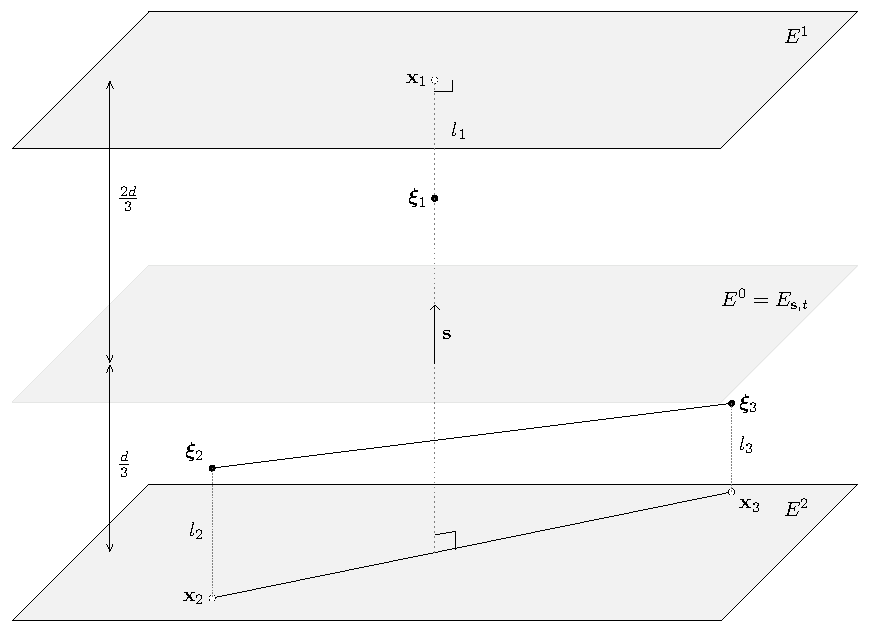
\includegraphics[width=0.95\textwidth]{figures/constraint_handling/three_point_interwell_problem.pdf}
	\caption{Three point problem}
	\label{fig:three_point_problem}
\end{figure}
%
We solve
\begin{align}
\min_{ \textbf{s} \in \mathbb{S}^2, t \in \mathbb{R}} F(\textbf{s},t) = \min_{ \textbf{s} \in \mathbb{S}^2, t \in \mathbb{R}}  \frac{1}{2} \sum_{i=1}^3 l_i(\textbf{s},t)^2,
\label{interwell_3point_problem}
\end{align}

where the lengths of the projections, $l_i$, are given by
%
\begin{align}
l_1(\textbf{s},t) &=  \langle \textbf{s}, \boldsymbol{\xi}_1 \rangle - t  - \frac{2d}{3}, \\
l_2(\textbf{s},t) &=  \langle \textbf{s}, \boldsymbol{\xi}_2 \rangle - t  + \frac{d}{3}, \\
l_3(\textbf{s},t) &=  \langle \textbf{s}, \boldsymbol{\xi}_3 \rangle - t  + \frac{d}{3}.
\label{eq:interwell_lengths_3p}
\end{align}
%
Again we minimize $F$ with respect to $t$ to get
\begin{align}
t &= \frac{1}{3} \sum_{i=1}^3 \langle \boldsymbol{\xi}_i,\textbf{s} \rangle.
\label{eq:three_point_t}
\end{align} 
Introducing the shifted variables
\begin{equation}
\hat{\boldsymbol{\xi}}_i = \boldsymbol{\xi}_i - \frac{1}{3} \sum_{i=1}^3 \boldsymbol{\xi}_i
\end{equation}
and using the value for $t$ found in \eqref{eq:three_point_t} and inserting these into
\eqref{interwell_3point_problem} we obtain the simplified problem
%
\begin{align}
\min_{ \textbf{s} \in \mathbb{S}^2, t \in \mathbb{R}} F(\textbf{s},t) = \min_{ \textbf{s} \in \mathbb{S}^2} \frac{1}{2} \sum_{i=1}^3 \hat{l}_i(\textbf{s})^2,
\label{interwell_3point_problem_shifted}
\end{align}
%
where 
%
\begin{align}
\hat{l}_1(\textbf{s},t) &=  \langle \textbf{s}, \hat{\boldsymbol{\xi}}_1 \rangle - \frac{2d}{3}, \\
\hat{l}_2(\textbf{s},t) &=  \langle \textbf{s}, \hat{\boldsymbol{\xi}}_2 \rangle + \frac{d}{3}, \\
\hat{l}_3(\textbf{s},t) &=  \langle \textbf{s}, \hat{\boldsymbol{\xi}}_3 \rangle + \frac{d}{3}.
\label{eq:interwell_lengths_3p_shifted}
\end{align}
%
We differentiate $F$ with respect to $\textbf{s}$ which gives
%
\begin{equation}
\frac{\partial F}{\partial \textbf{s}} (\textbf{s}) =  \sum_{i=1}^3 (\hat{\boldsymbol{\xi}}_i \otimes \hat{\boldsymbol{\xi}}_i)\textbf{s}
- \frac{2d}{3}\hat{\boldsymbol{\xi}}_1 + \frac{d}{3}(\hat{\boldsymbol{\xi}}_2 + \hat{\boldsymbol{\xi}}_3).
\end{equation}
%
A vector $\textbf{s}$ vector satisfies the necessary KKT conditions if it solves \eqref{eq:interwell_matrix} with
%
\begin{equation}
A = \sum_{i=1}^3 \hat{\boldsymbol{\xi}}_i \otimes \hat{\boldsymbol{\xi}}_i \quad \text{and} \quad 
b = \frac{2d}{3}\hat{\boldsymbol{\xi}}_1 - \frac{d}{3}(\hat{\boldsymbol{\xi}}_2 - \hat{\boldsymbol{\xi}}_3).
\label{eq:A_b_three_points}
\end{equation}
%
Solving \eqref{eq:interwell_matrix} can be done in exactly the same way
as described in the four-point case.
%
%
\subsection{Two-point solution}
%
If the two points are too close to each other they need to be moved
as little as possible away from each other so that they are a minimum
distance $d$ apart. This problem is identical to solving the well length 
constraint in equation \eqref{eq:well_length} with $L_{\min} = d$ and
$L_{\max} = \infty$.
%
\subsection{Complete inter-well distance constraint solution}
%
We have solved the two-, three-, and four-point problems individually and
combining them is the solution to the complete inter-well distance problem.
Below follows a pseudo code of the algorithm that solves the complete
inter-well distance problem. Note that by point we mean an endpoint of
a line segment.
%
\begin{algorithm}[H]
\caption{Inter-well distance projection}\label{alg:interwell_distance}
\begin{algorithmic}[1]
\Procedure{Project line segments to feasible space}{}
\State Get four initial points
\State
\For {all subsets with two points from different line segments}
\State Optimal projection of two points
	\If{Four point configuration satisfies inter-well constraint}
		\State Calculate movement cost and save configuration
	\EndIf
\EndFor

\State
\If{any two point solution satisfies constraints}
\State return best two point solution
\EndIf

\State
\For {all subsets with three points}
\State Optimal projection of three points
	\If{Four point configuration satisfies inter-well constraint}
		\State Calculate movement cost and save configuration
	\EndIf
\EndFor

\State
\If{any three point solution satisfies constraints}
\State return best three point solution
\EndIf
\State

\State Optimal projection of four points
\State return four point solution

\EndProcedure
\end{algorithmic}
\end{algorithm}
%
%